\chapter{Fluvial Generative Adversarial Network Architecture}\label{Appendix:FluvGAN_Architecture}
This appendix provides a comprehensive technical specification of the 3D \gls{fluvgan} framework utilized in this research. Section~\ref{sec:app_arch_overview} presents the macro-architectural design and its relation to the methodology described in Chapter~\ref{Ch:Methodology}. Section~\ref{sec:app_generator_arch} details the layer-by-layer parameterization of the 3D DeepGenerator network~($\mathbf{G}$), while Section~\ref{sec:app_discriminator_arch} outlines the 3D DeepDiscriminator network~($\mathbf{D}$). Finally, Section~\ref{sec:app_resblocks_design} elaborates on the residual block mechanics and training convergence dynamics.

\section{Architectural Overview}\label{sec:app_arch_overview}
The generative framework is adapted from the 3D \gls{dcgan} architecture introduced by~\textcite{rongier2025afluvgan}. As described in Section~\ref{Subsec:Model_architecture}, the model processes 3D categorical facies data formatted as multi-channel tensors of dimension $C \times 32 \times 128 \times 128$, where $C$ represents the number of one-hot encoded facies channels ($C=3$ for the upscaled dataset and $C=9$ for the high-fidelity dataset). The macro-level schematic of the generator and discriminator pipelines is illustrated in Figure~\ref{fig:fluvgan_architecture} (Chapter~\ref{Ch:Methodology}).

The generator synthesizes 3D facies volumes by expanding an initial low-dimensional stochastic latent vector through a sequence of progressive 3D transposed convolutions and residual upscaling blocks. Symmetrically, the discriminator evaluates candidate volumes (either authentic training samples from FLUMY or synthetic generations) by contracting the 3D grid through downscaling residual blocks to compute a single scalar logit. Both networks leverage double residual blocks (\say{Double ResBlocks}) at each spatial scale to ensure high representational capacity and preserve gradient stability throughout deep 3D backpropagation.

\section{Generator Architecture (DeepGenerator3d)}\label{sec:app_generator_arch}
The generator network~($\mathbf{G}$) transforms an isotropic Gaussian latent noise vector $\mathbf{z}^* \in \mathbb{R}^{100}$, with $\mathbf{z}^* \sim \mathcal{N}(0, \mathbf{I})$, into a discrete 3D categorical facies realization. The complete layer configuration is summarized in Table~\ref{tab:best_generator_architecture} and proceeds through six progressive scales:

\begin{enumerate}
    \item \textbf{Latent Projection (Scale~1):} The 100-dimensional latent vector is projected via a 3D transposed convolutional block (\texttt{ConvBlockTranspose3d}) into an initial 3D feature volume of dimension $1024 \times 4 \times 4 \times 4$. This dense projection comprises 6,553,600 trainable parameters, establishing the base spatial representation.
    \item \textbf{Progressive Upscaling (Scales~2 to~6):} Spatial dimensions are expanded stepwise from $4 \times 4 \times 4$ to the final grid resolution of $32 \times 128 \times 128$. Each spatial scale incorporates a paired residual block structure:
    \begin{itemize}
        \item An upscaling residual block (\texttt{DeepResBlockUpscale3d}) that performs spatial interpolation and transposed convolution while adjusting feature channel depth;
        \item A standard residual block (\texttt{DeepResBlock3d}) operating at the newly upscaled resolution to refine feature representations without modifying spatial dimensions.
    \end{itemize}
    Across Scales~2 to~6, the feature channel density is progressively halved ($1024 \to 512 \to 256 \to 128 \to 64$), managing memory constraints while increasing spatial fidelity.
    \item \textbf{Output Layer \& Categorical Discretization:} The final feature map of size $64 \times 32 \times 128 \times 128$ is processed through a 3D Batch Normalization layer paired with a LeakyReLU activation function, before passing into a final 3D convolution (\texttt{ConvBlock3d}) that projects the 64 feature maps into the target $C$ facies channels ($C=9$ or $C=3$).
\end{enumerate}

To maintain bounded gradients during adversarial training, the output layer utilizes a hyperbolic tangent ($\tanh$) activation function, bounding the continuous channel outputs to $[-1, 1]$. To convert these continuous channel activations back into discrete geological facies, a channel-wise $\operatorname{argmax}$ operation is applied:
\begin{equation}
    \text{Facies}(z, y, x) = \arg\max_{c \in \{1, \dots, C\}} G(\mathbf{z}^*)_{c, z, y, x}
\end{equation}
resulting in a final 3D volume of size $32 \times 128 \times 128$ populated by discrete integer facies labels. In total, the generator contains 21,054,112 trainable parameters (Table~\ref{tab:best_generator_architecture}).

\begin{table}[htbp]
    \centering
    \renewcommand{\arraystretch}{1.2}
    \begin{tabular}{p{0.45\textwidth}cc}
        \hline
        \textbf{Layer / Block Type} & \textbf{Output Shape} & \textbf{Param \#} \\
        \hline
        ConvBlockTranspose3d (Scale 1) & [1, 1024, 4, 4, 4] & 6,553,600 \\
        DeepResBlockUpscale3d (Scale 2) & [1, 1024, 8, 8, 8] & 4,066,816 \\
        DeepResBlock3d (Scale 2) & [1, 1024, 8, 8, 8] & 4,066,816 \\
        DeepResBlockUpscale3d (Scale 3) & [1, 512, 16, 16, 16] & 3,935,744 \\
        DeepResBlock3d (Scale 3) & [1, 512, 16, 16, 16] & 1,017,600 \\
        DeepResBlockUpscale3d (Scale 4) & [1, 256, 32, 32, 32] & 984,832 \\
        DeepResBlock3d (Scale 4) & [1, 256, 32, 32, 32] & 254,848 \\
        DeepResBlockUpscale3d (Scale 5) & [1, 128, 32, 64, 64] & 99,200 \\
        DeepResBlock3d (Scale 5) & [1, 128, 32, 64, 64] & 27,072 \\
        DeepResBlockUpscale3d (Scale 6) & [1, 64, 32, 128, 128] & 25,024 \\
        DeepResBlock3d (Scale 6) & [1, 64, 32, 128, 128] & 6,880 \\
        BatchNorm3d + LeakyReLU & [1, 64, 32, 128, 128] & 128 \\
        ConvBlock3d (Output) & [1, 9, 32, 128, 128] & 15,552 \\
        \hline
        \textbf{Total Trainable Parameters} & \multicolumn{2}{c}{\textbf{21,054,112}} \\
        \hline
    \end{tabular}
    \caption{Detailed architectural specifications and layer parameters for the DeepGenerator3d network.}
    \label{tab:best_generator_architecture}
\end{table}

\section{Discriminator Architecture (DeepDiscriminator3d)}\label{sec:app_discriminator_arch}
The discriminator network~($\mathbf{D}$) functions as a binary classifier, determining whether an input volume of dimension $C \times 32 \times 128 \times 128$ represents an authentic FLUMY simulation or a synthetic realization generated by $\mathbf{G}$. The structural hierarchy is outlined in Table~\ref{tab:best_discriminator_architecture}:

\begin{enumerate}
    \item \textbf{Input Feature Extraction (Scale~1):} The incoming one-hot encoded tensor is processed through an initial 3D convolutional block (\texttt{ConvBlock3d}), projecting the $C$ facies channels into 64 feature maps at the full grid resolution ($32 \times 128 \times 128$).
    \item \textbf{Progressive Downscaling (Scales~2 to~6):} The spatial dimensions are compressed across five consecutive stages ($32 \times 128 \times 128 \to 16 \times 64 \times 64 \to 8 \times 32 \times 32 \to 4 \times 16 \times 16 \to 4 \times 8 \times 8 \to 4 \times 4 \times 4$). In symmetry with the generator, each scale consists of:
    \begin{itemize}
        \item A downscaling residual block (\texttt{DeepResBlockDownscale3d}) that halves spatial resolution while expanding feature depth;
        \item A secondary residual block (\texttt{DeepResBlock3d}) that refines spatial correlation patterns.
    \end{itemize}
    Feature channels are progressively doubled from 64 up to 1024, enabling the discriminator to capture both fine-scale facies transitions and macro-scale channel body geometry.
    \item \textbf{Classification Output:} The final $1024 \times 4 \times 4 \times 4$ feature representation is activated via LeakyReLU and flattened into a linear layer (\texttt{LinearBlock}), producing a single scalar logit $D(\mathbf{x})$.
\end{enumerate}

The discriminator comprises 7,656,129 trainable parameters (Table~\ref{tab:best_discriminator_architecture}), providing a parameter ratio of approximately $1:2.75$ relative to the generator. This ratio ensures that the discriminator provides informative gradient feedback without prematurely overpowering the generator.

\begin{table}[htbp]
    \centering
    \renewcommand{\arraystretch}{1.2}
    \begin{tabular}{p{0.45\textwidth}cc}
        \hline
        \textbf{Layer / Block Type} & \textbf{Output Shape} & \textbf{Param \#} \\
        \hline
        ConvBlock3d (Input) & [1, 64, 32, 128, 128] & 15,552 \\
        DeepResBlockDownscale3d (Scale 2) & [1, 128, 16, 64, 64] & 20,992 \\
        DeepResBlock3d (Scale 2) & [1, 128, 16, 64, 64] & 63,488 \\
        DeepResBlockDownscale3d (Scale 3) & [1, 256, 8, 32, 32] & 83,968 \\
        DeepResBlock3d (Scale 3) & [1, 256, 8, 32, 32] & 253,952 \\
        DeepResBlockDownscale3d (Scale 4) & [1, 512, 4, 16, 16] & 335,872 \\
        DeepResBlock3d (Scale 4) & [1, 512, 4, 16, 16] & 1,015,808 \\
        DeepResBlockDownscale3d (Scale 5) & [1, 1024, 4, 8, 8] & 753,664 \\
        DeepResBlock3d (Scale 5) & [1, 1024, 4, 8, 8] & 1,703,936 \\
        DeepResBlockDownscale3d (Scale 6) & [1, 1024, 4, 4, 4] & 1,703,936 \\
        DeepResBlock3d (Scale 6) & [1, 1024, 4, 4, 4] & 1,703,936 \\
        LeakyReLU & [1, 1024, 4, 4, 4] & 0 \\
        LinearBlock (Output Prediction) & [1, 1] & 1,025 \\
        \hline
        \textbf{Total Trainable Parameters} & \multicolumn{2}{c}{\textbf{7,656,129}} \\
        \hline
    \end{tabular}
    \caption{Detailed architectural specifications and layer parameters for the DeepDiscriminator3d network.}
    \label{tab:best_discriminator_architecture}
\end{table}

\section{Residual Block Mechanics and Convergence Dynamics}\label{sec:app_resblocks_design}
Stacking standard 3D convolutional layers in deep generative models often leads to vanishing gradients and mode collapse, exacerbated by the cubic parameter growth in 3D volumes. To mitigate this instability, the \gls{fluvgan} architecture integrates residual connections throughout both networks~\parencite{he2016deep}. Each residual unit evaluates:
\begin{equation}
    \mathbf{y} = \mathcal{F}(\mathbf{x}, \{\mathcal{W}_i\}) + \mathcal{W}_s \mathbf{x}
\end{equation}
where $\mathbf{x}$ and $\mathbf{y}$ denote input and output tensors, $\mathcal{F}$ represents the residual transformation consisting of paired 3D convolutions, 3D batch normalization, and LeakyReLU activations, and $\mathcal{W}_s$ represents an optional linear $1 \times 1 \times 1$ projection applied exclusively when matching channel dimensions during spatial transitions.

The incorporation of double residual blocks at each spatial scale provides the expressive capacity necessary to learn complex fluvial geometries (such as channel sinuosity and point bar accretion) while maintaining smooth gradient flow. Figure~\ref{fig:msswd_mds_best_models} illustrates the structural convergence of this optimized architecture over training epochs, visualised via \gls{mds} of \gls{msswd} values. Between Epochs 25 and 100, the generated distribution shifts progressively toward the authentic reference data cluster, demonstrating that the residual design stabilizes training and captures the multi-scale spatial characteristics of the training datasets.

% \begin{figure}[htbp]
%     \centering
%     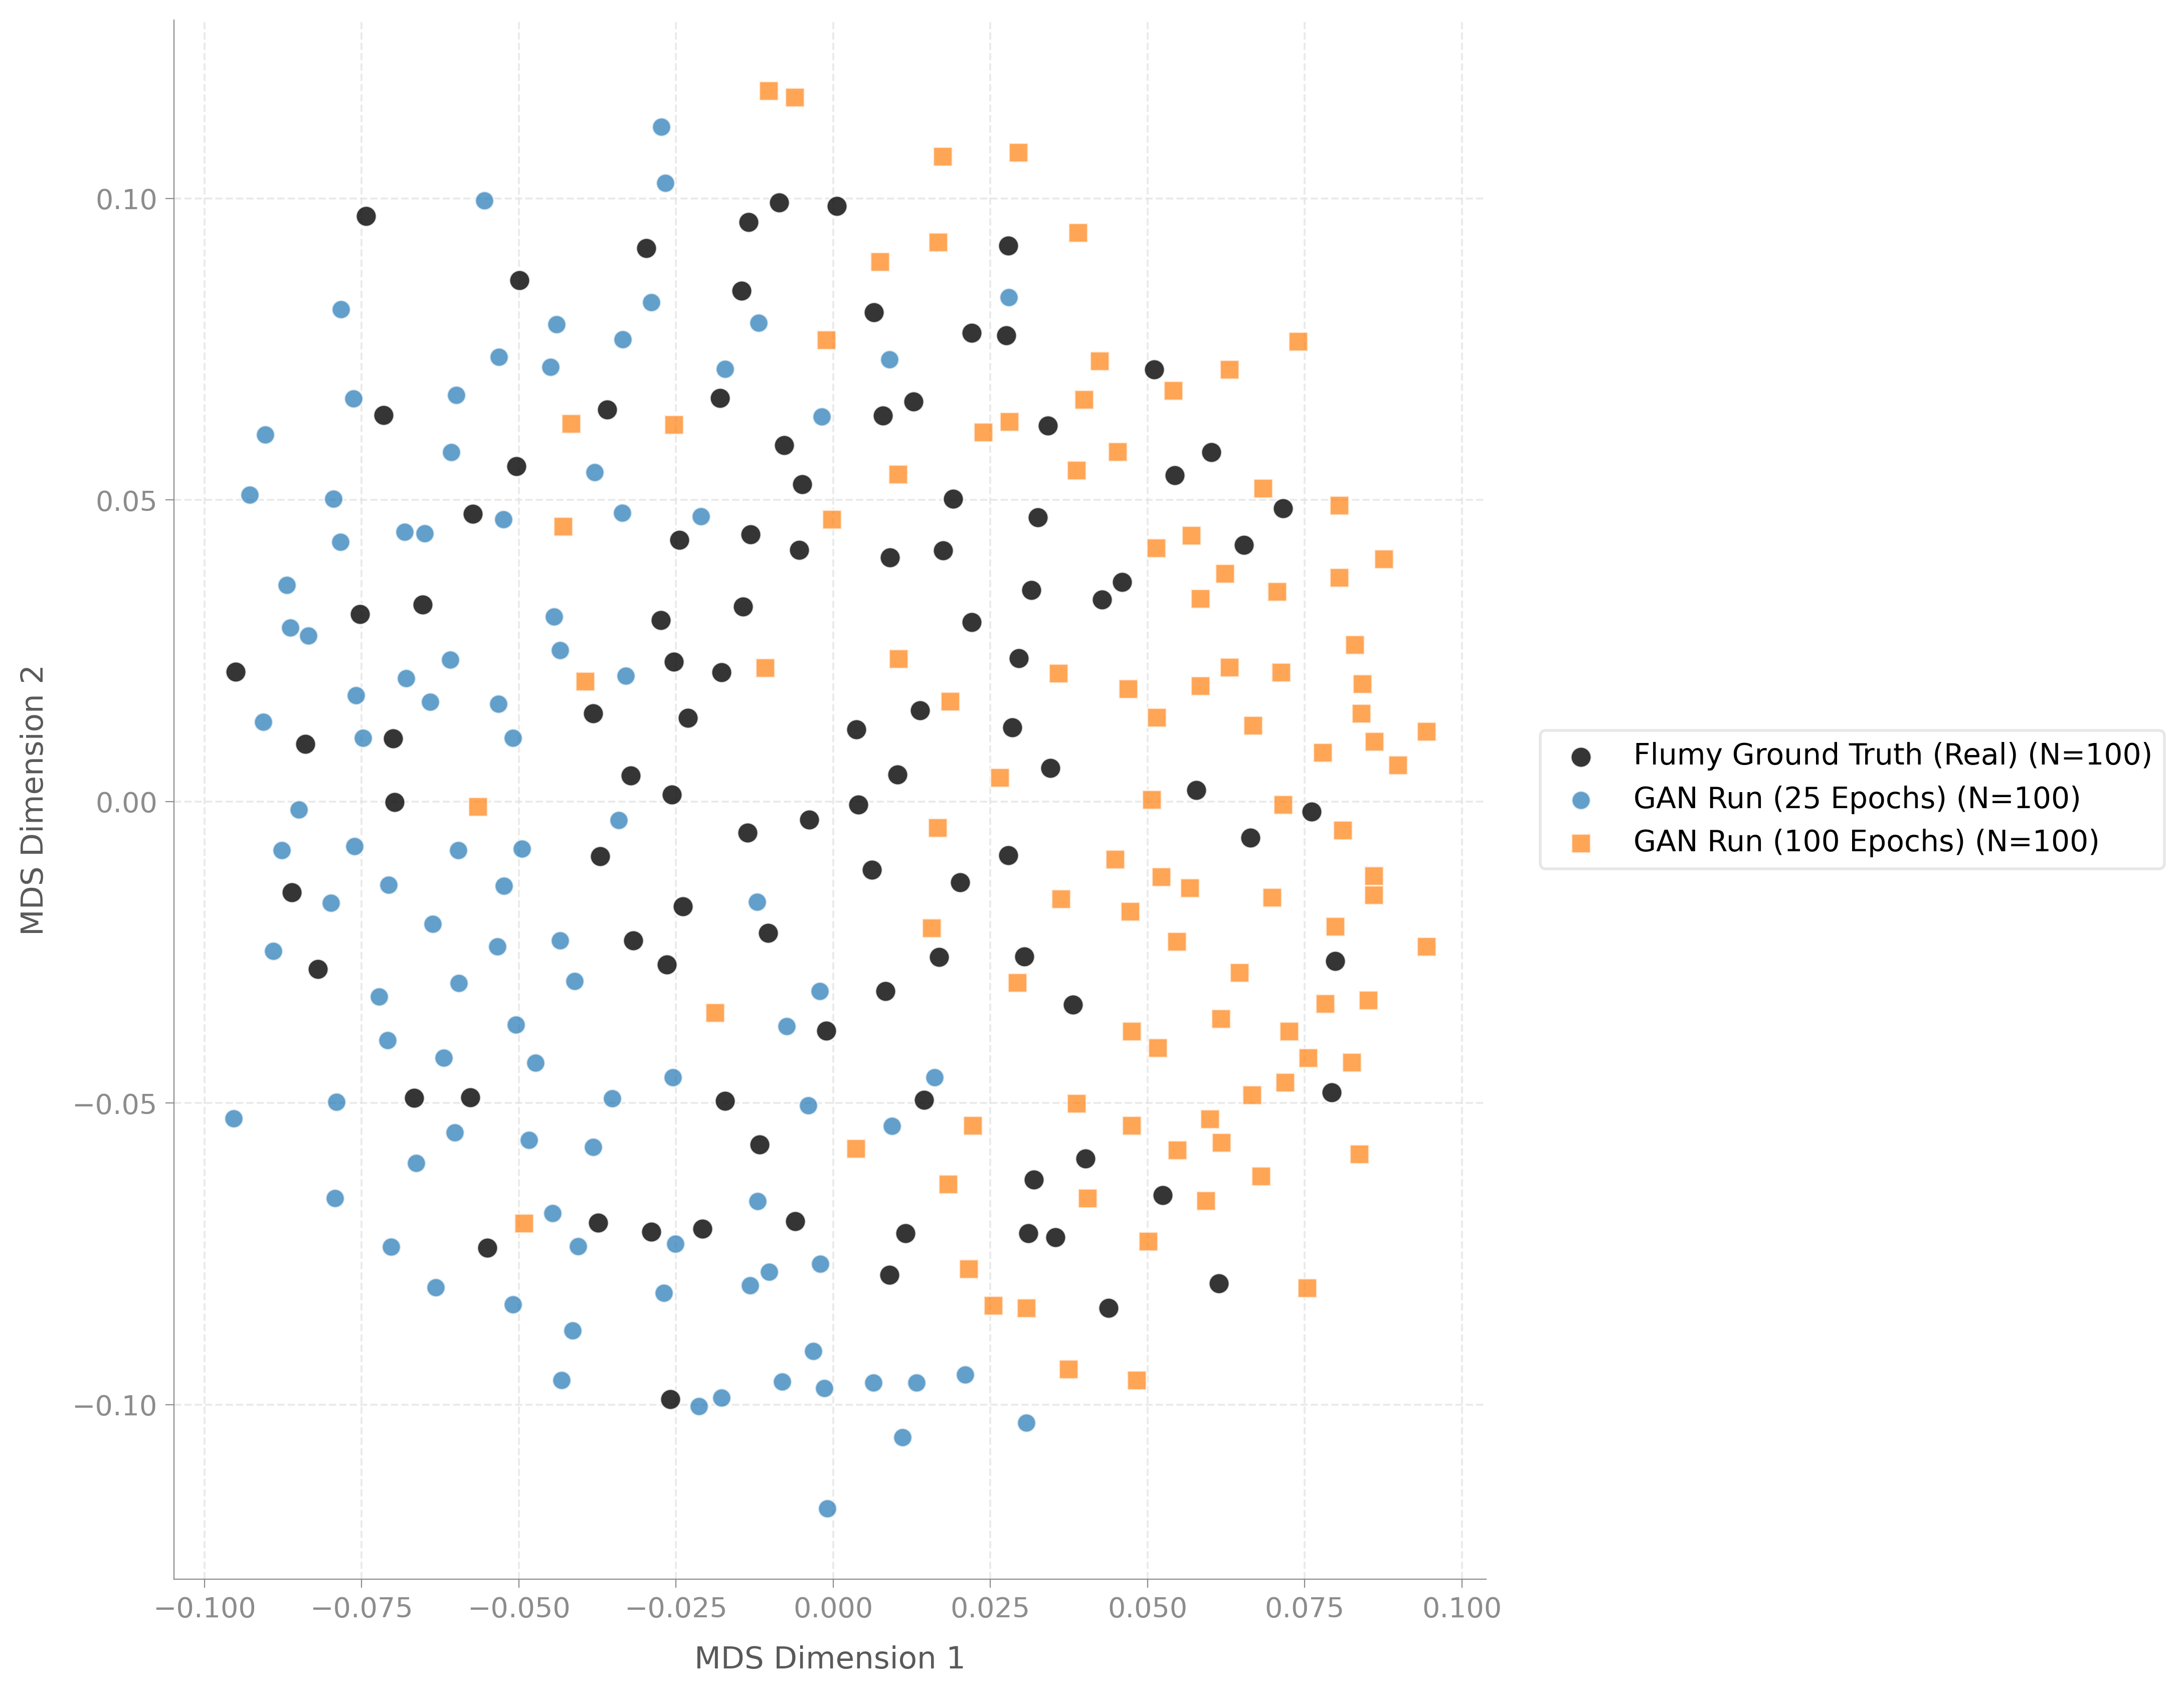
\includegraphics[width=0.80\textwidth]{figures/results/cgan_unconstrained_performance/ms_swd_mds_plot.png}
%     \caption{\glsentryshort{mds} plot of the \glsentryshort{msswd} values computed for the test dataset, illustrating the distribution shift and clustering behaviour of the model 5 architecture between 25 and 100 training epochs.}
%     \label{fig:msswd_mds_best_models}
% \end{figure}